\documentclass[twocolumn, 10pt]{article}

\usepackage{geometry}
\geometry{
	a4paper,
	total={6.85in, 9.92in},
	left=0.71in,
	top=0.63in,
}
\usepackage{caption}
\usepackage{enumitem}
\usepackage[utf8]{inputenc}
\usepackage{hyperref}
\usepackage{graphicx}
\usepackage{listings}
\usepackage{lipsum} % XXX: Remove that
\usepackage{titlesec}
\usepackage{url}
\usepackage{xcolor} % XXX: Remove that
% \usepackage{newunicodechar}

% \usepackage{sansmathfonts}
% \usepackage[T1]{fontenc}
% \renewcommand*\familydefault{\sfdefault} %% Only if the base font of the document is to be sans serif
% \renewcommand{\familydefault}{\ttdefault}

% unicodes styling
% \DeclareUnicodeCharacter{2014}{\dash}
% unicodes - end
\pagenumbering{gobble}

% listing styling
\definecolor{commentsColor}{rgb}{0.497495, 0.497587, 0.497464}
\definecolor{identifierColor}{rgb}{0.9, 0.01, 0.9}
\definecolor{keywordsColor}{rgb}{0.000000, 0.000000, 0.635294}
\definecolor{stringColor}{rgb}{0.558215, 0.000000, 0.135316}

\lstset{
    abovecaptionskip=\vspace{0pt},
    belowcaptionskip=\vspace{0pt},
    backgroundcolor=\color{yellow!10},
    basicstyle=\ttfamily\footnotesize,
    breakatwhitespace=true,
    breaklines=true,
    postbreak=\mbox{\textcolor{red}{$\hookrightarrow$}\space},
    commentstyle=\color{commentsColor}\textit,
    escapeinside={\%*}{*)},
    extendedchars=false,
    frame=single,
    frameround=tftf,
    framerule=0pt,
    framexbottommargin=0pt,
    framextopmargin=0pt,
    framexleftmargin=0pt,
    ndkeywordstyle=\color{identifierColor}\bfseries,
    inputencoding=utf8,
    keywordstyle=\color{keywordsColor}\bfseries,
    numbers=none,
    numberstyle=\footnotesize,
    rulecolor=\color{black!30},
    stringstyle=\color{stringColor}\bfseries,
    showspaces=false,
    tabsize=2pt,
    title=\lstname,
    breaklines=true,
    postbreak=\mbox{\textcolor{red}{$\hookrightarrow$}\space}
}

\lstdefinestyle{c}{language=c,
    morekeywords={uint32_t, int32_t, uint8_t, printf, size_t},
        backgroundcolor=\color{clr-background},
        basicstyle=\color{clr-text}, % any text
        stringstyle=\color{clr-string},
        identifierstyle=\color{clr-variable}, % about not directive, comment, string or known type
        commentstyle=\color{clr-comment},
        directivestyle=\color{clr-preprocessor}, % preprocessor commands
        % listings doesn't differentiate between types and keywords (e.g. int vs return)
        % use the user types color
        keywordstyle=\color{clr-type},
        keywordstyle={[2]\color{clr-constant}}, % you'll need to define these or use a custom language
        tabsize=2
}
% \lstdefinestyle{sh}{
%   language=sh
% }

\lstdefinestyle{python}{language=python,
  morekeywords={uint32_t, int32_t, uint8_t, printf, size_t},
      backgroundcolor=\color{clr-background},
      basicstyle=\color{clr-text}, % any text
      stringstyle=\color{clr-string},
      identifierstyle=\color{clr-variable}, % about not directive, comment, string or known type
      commentstyle=\color{clr-comment},
      directivestyle=\color{clr-preprocessor}, % preprocessor commands
      % listings doesn't differentiate between types and keywords (e.g. int vs return)
      % use the user types color
      keywordstyle=\color{clr-type},
      keywordstyle={[2]\color{clr-constant}}, % you'll need to define these or use a custom language
      tabsize=2
}
\DeclareCaptionFormat{listing}{\rule{]\dimexpr\textwidth+17pt\relax}{0.4pt}\vskip1pt#1#2#3}
% listing - end
\usepackage{etoolbox}
\patchcmd{\thebibliography}{\subsection*{\refname}}{}{}{}

\titlespacing{\section}{0pt}{\parskip}{-\parskip}
\titlespacing{\subsection}{0pt}{\parskip}{-\parskip}

\vspace{-\baselineskip}
\setlength{\parindent}{0pt}
\DeclareCaptionLabelFormat{filelabel}{File~#2}
\captionsetup[lstlisting]{labelformat=filelabel}

\title{RPI4 remote debug recipe!}
\author{Kajetan Brzuszczak}

\makeatletter
\newcommand{\fsize}{\f@size pt }
\newcommand{\textFontName}{\f@family}
\renewcommand{\maketitle}{
\begin{flushleft}
{\noindent\Huge\bf\@title}\break
\end{flushleft}
}
\makeatother

\begin{document}
\maketitle

Tools: \textit{RPI4, C++, VSCode, CMake, Linux}

\subsection*{Minimal project structure}
\normalsize

Before we start with the main topic, a few files need to be created.
Thus, create a project which should match at least the following tree directory:
\begin{lstlisting}[language=sh,caption={},backgroundcolor=\color{gray!10}]
.
-> .vscode
   -> launch.json
   -> settings.json
-> src
    -> main.cc
-> CMakeLists.txt
-> rpi4.toolchain.cmake
\end{lstlisting}

The content of the above structure can be found by the reader in the exeternal repo\cite{bib:example}.
Once you get it, replace the following paths with your own favorite paths as needed
\begin{enumerate}
  \item workspace: \\
        \textit{/mnt/d/programming/remote\_debug\_rpi/}
  \item image directory: \\
        \textit{/mnt/d/programming/x-compile-os/}
\end{enumerate}

\subsection*{Environment}
Install x-compile and indexing tools
\begin{lstlisting}[backgroundcolor=\color{gray!10},caption={}]
sudo apt install -y gcc-10-aarch64-linux-gnu g++-10-aarch64-linux-gnu gdb-multiarch clangd
\end{lstlisting}

Dump your RPI SD card or download a proper flash image\cite{bib:rpi-images} as \textit{rpi\_img}.
Then, you are ready to configure your system and install the plugin for debugging.

\begin{lstlisting}[language=sh,backgroundcolor=\color{gray!10},breaklines=true,escapechar=|,caption={}]]
unxz --keep <rpi_img>.img.xz
mkdir -p /mnt/d/programming/x-compile-os/rpi4
sudo mount -v -o  offset=272629760  <rpi_img>.img.xz /mnt/d/programming/x-compile-os/rpi4

code --install-extension webfreak.debug
code --install-extension llvm-vs-code-extensions.vscode-clangd
\end{lstlisting}

\subsection*{Playground}
Now, compile the project and put the compiled binary on the raspberry.
\begin{lstlisting}[language=sh,breaklines=true,caption={},,escapechar=|,backgroundcolor=\color{gray!10}]
cmake -S . -B out_rpi -DCMAKE_EXPORT_COMPILE_COMMANDS=True -DCMAKE_BUILD_TYPE=Debug --toolchain rpi4.toolchain.cmake
cmake --build out_rpi -j7
scp out_rpi/debug_rpi rpi:|$\sim$|/
\end{lstlisting}

The final step is to run the binary using \textift{gdbserver}, and after that, run a debug session by attaching it in your VSCode (or by pressing the "\textbf{F5}" key).
\begin{lstlisting}[language=sh,breaklines=true,caption={},escapechar=|,backgroundcolor=\color{gray!10}]
# FROM RPI
gdbserver :9999 |$\sim$|/debug_rpi
\end{lstlisting}
Voilà! You have now become a driver.

\begin{figure}
  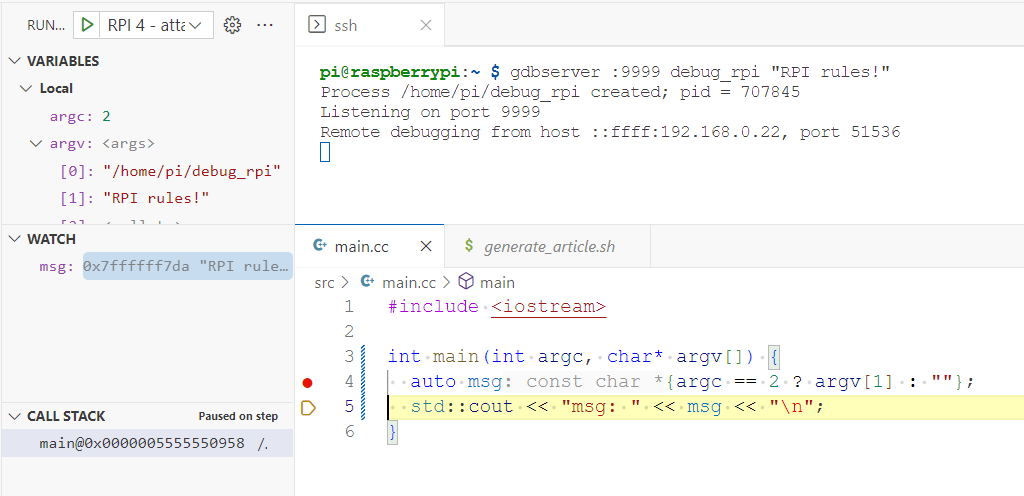
\includegraphics[width=\linewidth]{res/remote_debug_rpi_light.png}
  \caption*{VSCode attached to a remote app}
  \label{fig:debug}
\end{figure}

\subsection*{Further steps}
Being in sync with the image and the RPI is highly recommended.
  If any library is installed directly on the RPI, the image
  should be updated with the same copy. And until any platform-spefic header is used
  e.g. \mbox{\textit{linux/spi.h}} or \mbox{\textit{linux/gpio.h}}, the code should be compilable
  locally without additional effort.

With the current setup, you also get automatically generated \textit
  {compile\_commands.json} file utilized by \textit{clangd}
  \cite{bib:clangd} which provides code navigation and code completion.
  The same approach is appliccable even for quite large repositories,
  such as Chromium.

Last but not least, a major gain of remote debugging, not used here, is reducing
  the required disk usage by using \textit{stripped} binaries on the RPI while keeping a debuggable version on your PC.

\subsection*{Misses}
\begin{enumerate}
  \item rpi ip in the \textit{launch.json} file - hardcoded, seems the plugin does not support aliases,
        so it has to be replaced with your own RPI4 ip address
  \item port 9999 - I like the number, but your firewall might feel differently
  \item mounting offset - check \cite{bib:mounting-approach} out
\end{enumerate}

\subsection*{Caveats}
Things are gettting much more complicated when the project grows larger,
  libraries are distributed more widely, and it is compiled on a remote
  station using a virtual machine (e.g. \textit{qemu}). Eventually,
  your simple configuration may stop working. However,
  GDB provides commands that can help point to the correct places,
  such as \textit{set solib-search-path path} or
  \textit{set substitute-path from to} etc.\cite{bib:gdb-additional-configs}

\subsection*{References}
\begin{enumerate}[label={[\arabic*]}]
  \footnotesize
  \bibitem{bib:example} \url{https://github.com/HalfInner/remote_debug_rpi}
  \bibitem{bib:rpi-images} \url{https://www.raspberrypi.com/software/operating-systems/}
  \bibitem{bib:clangd} \url{https://clangd.llvm.org/}
  \bibitem{bib:mounting-approach} \url{https://raspberrypi.stackexchange.com/a/13138}
  \bibitem{bib:gdb-additional-configs} \url{https://sourceware.org/gdb/onlinedocs/gdb/Source-Path.html}
  \bibitem{bib:c++-rpi} \url{https://tttapa.github.io/Pages/Raspberry-Pi/C++-Development-RPiOS/index.html}
\end{enumerate}

% The font used is \textFontName

\end{document}
